\documentclass{beamer}
\author{Julius Elinson}
\usetheme{Frankfurt}
\usecolortheme{beaver}
\usepackage{multicol, amsmath,mathpazo}
\title{Image-Based Rock-Climbing Simulator}
\subtitle{Artificial Intelligence Final Project}
\institute{Harvey Mudd College \\CS 151}
\date{\today}

\beamertemplatenavigationsymbolsempty

\begin{document}
\frame{\titlepage}


\section{Problem}
\begin{frame}{Rock Climbing}
\begin{columns}

\begin{column}[T]{.5\linewidth}
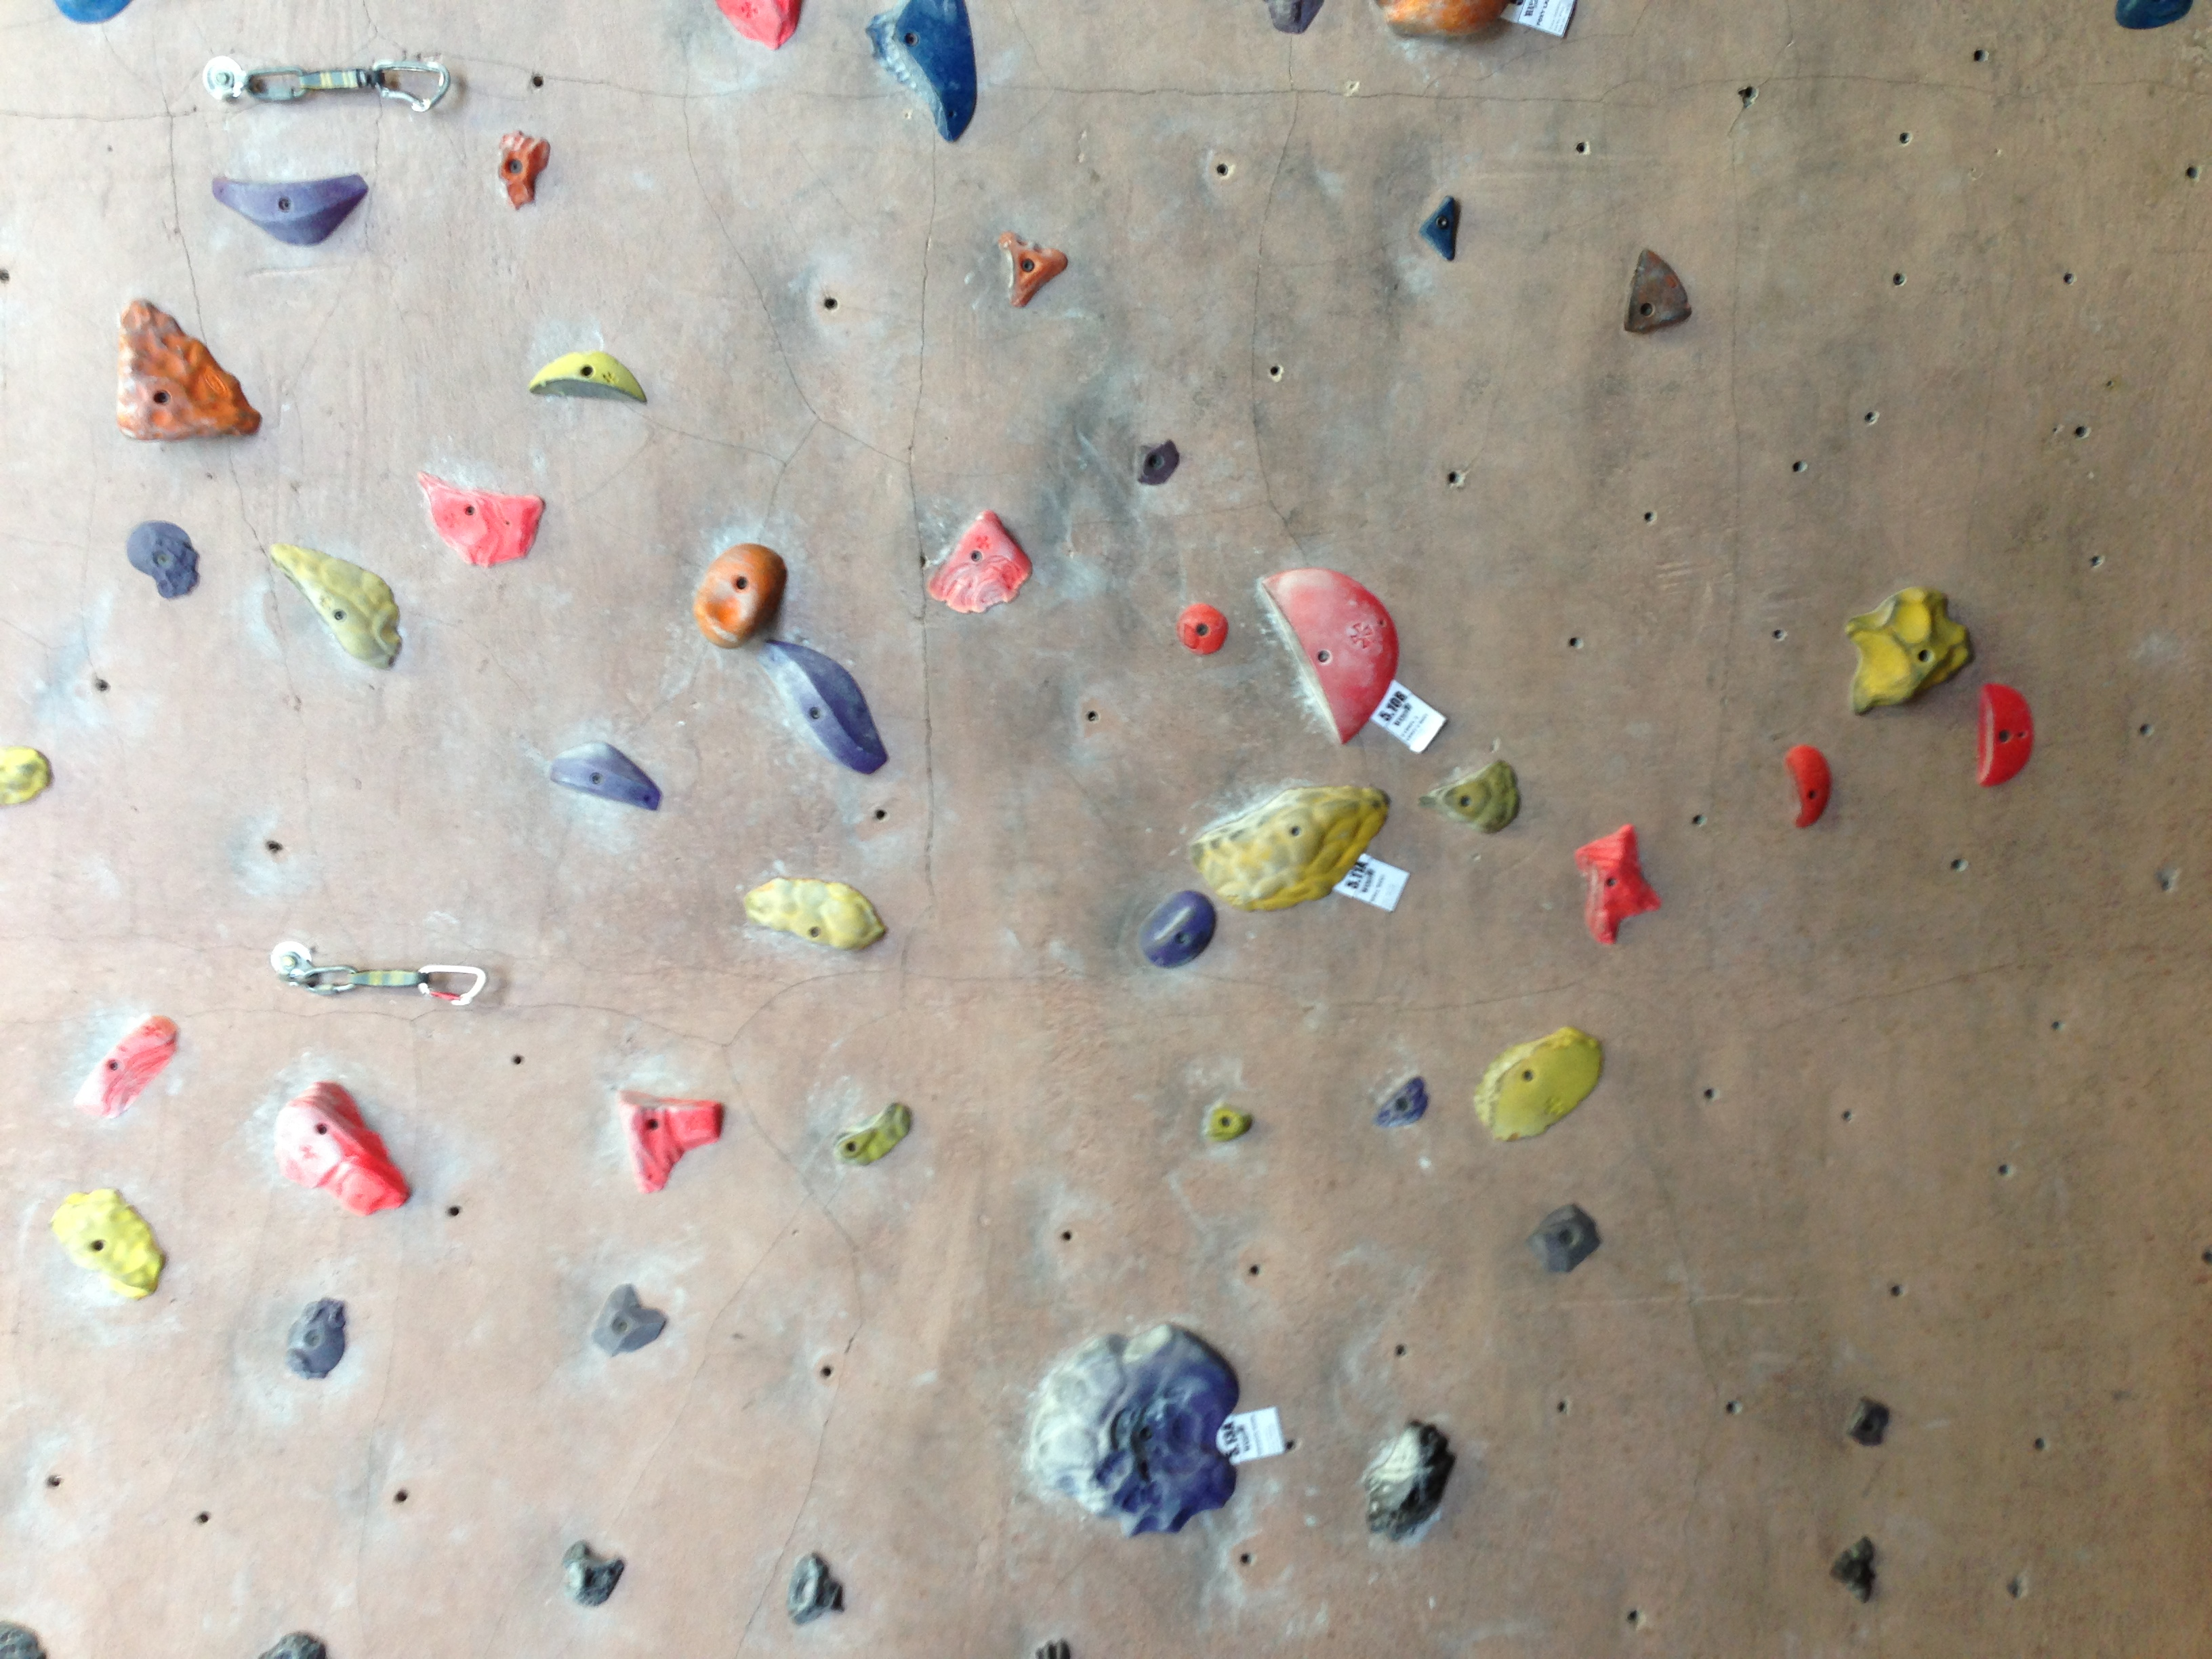
\includegraphics[height=\linewidth,angle=-90]{img/test2.JPG}
\end{column}
\pause
\begin{column}[T]{.6\linewidth}
\vspace{.8cm}
Problem Definition
\begin{itemize}
 \item Routes are color-delimited
 \item Use any subset of designated grips to get to the top
 \item Difficulty determined by size, spacing and surface properties of the grips
 \item Climbers have to determine a path
\end{itemize}

\end{column}

\end{columns}
\end{frame}


\begin{frame}{Rock Climbing}
\begin{columns}

\begin{column}[T]{.5\linewidth}
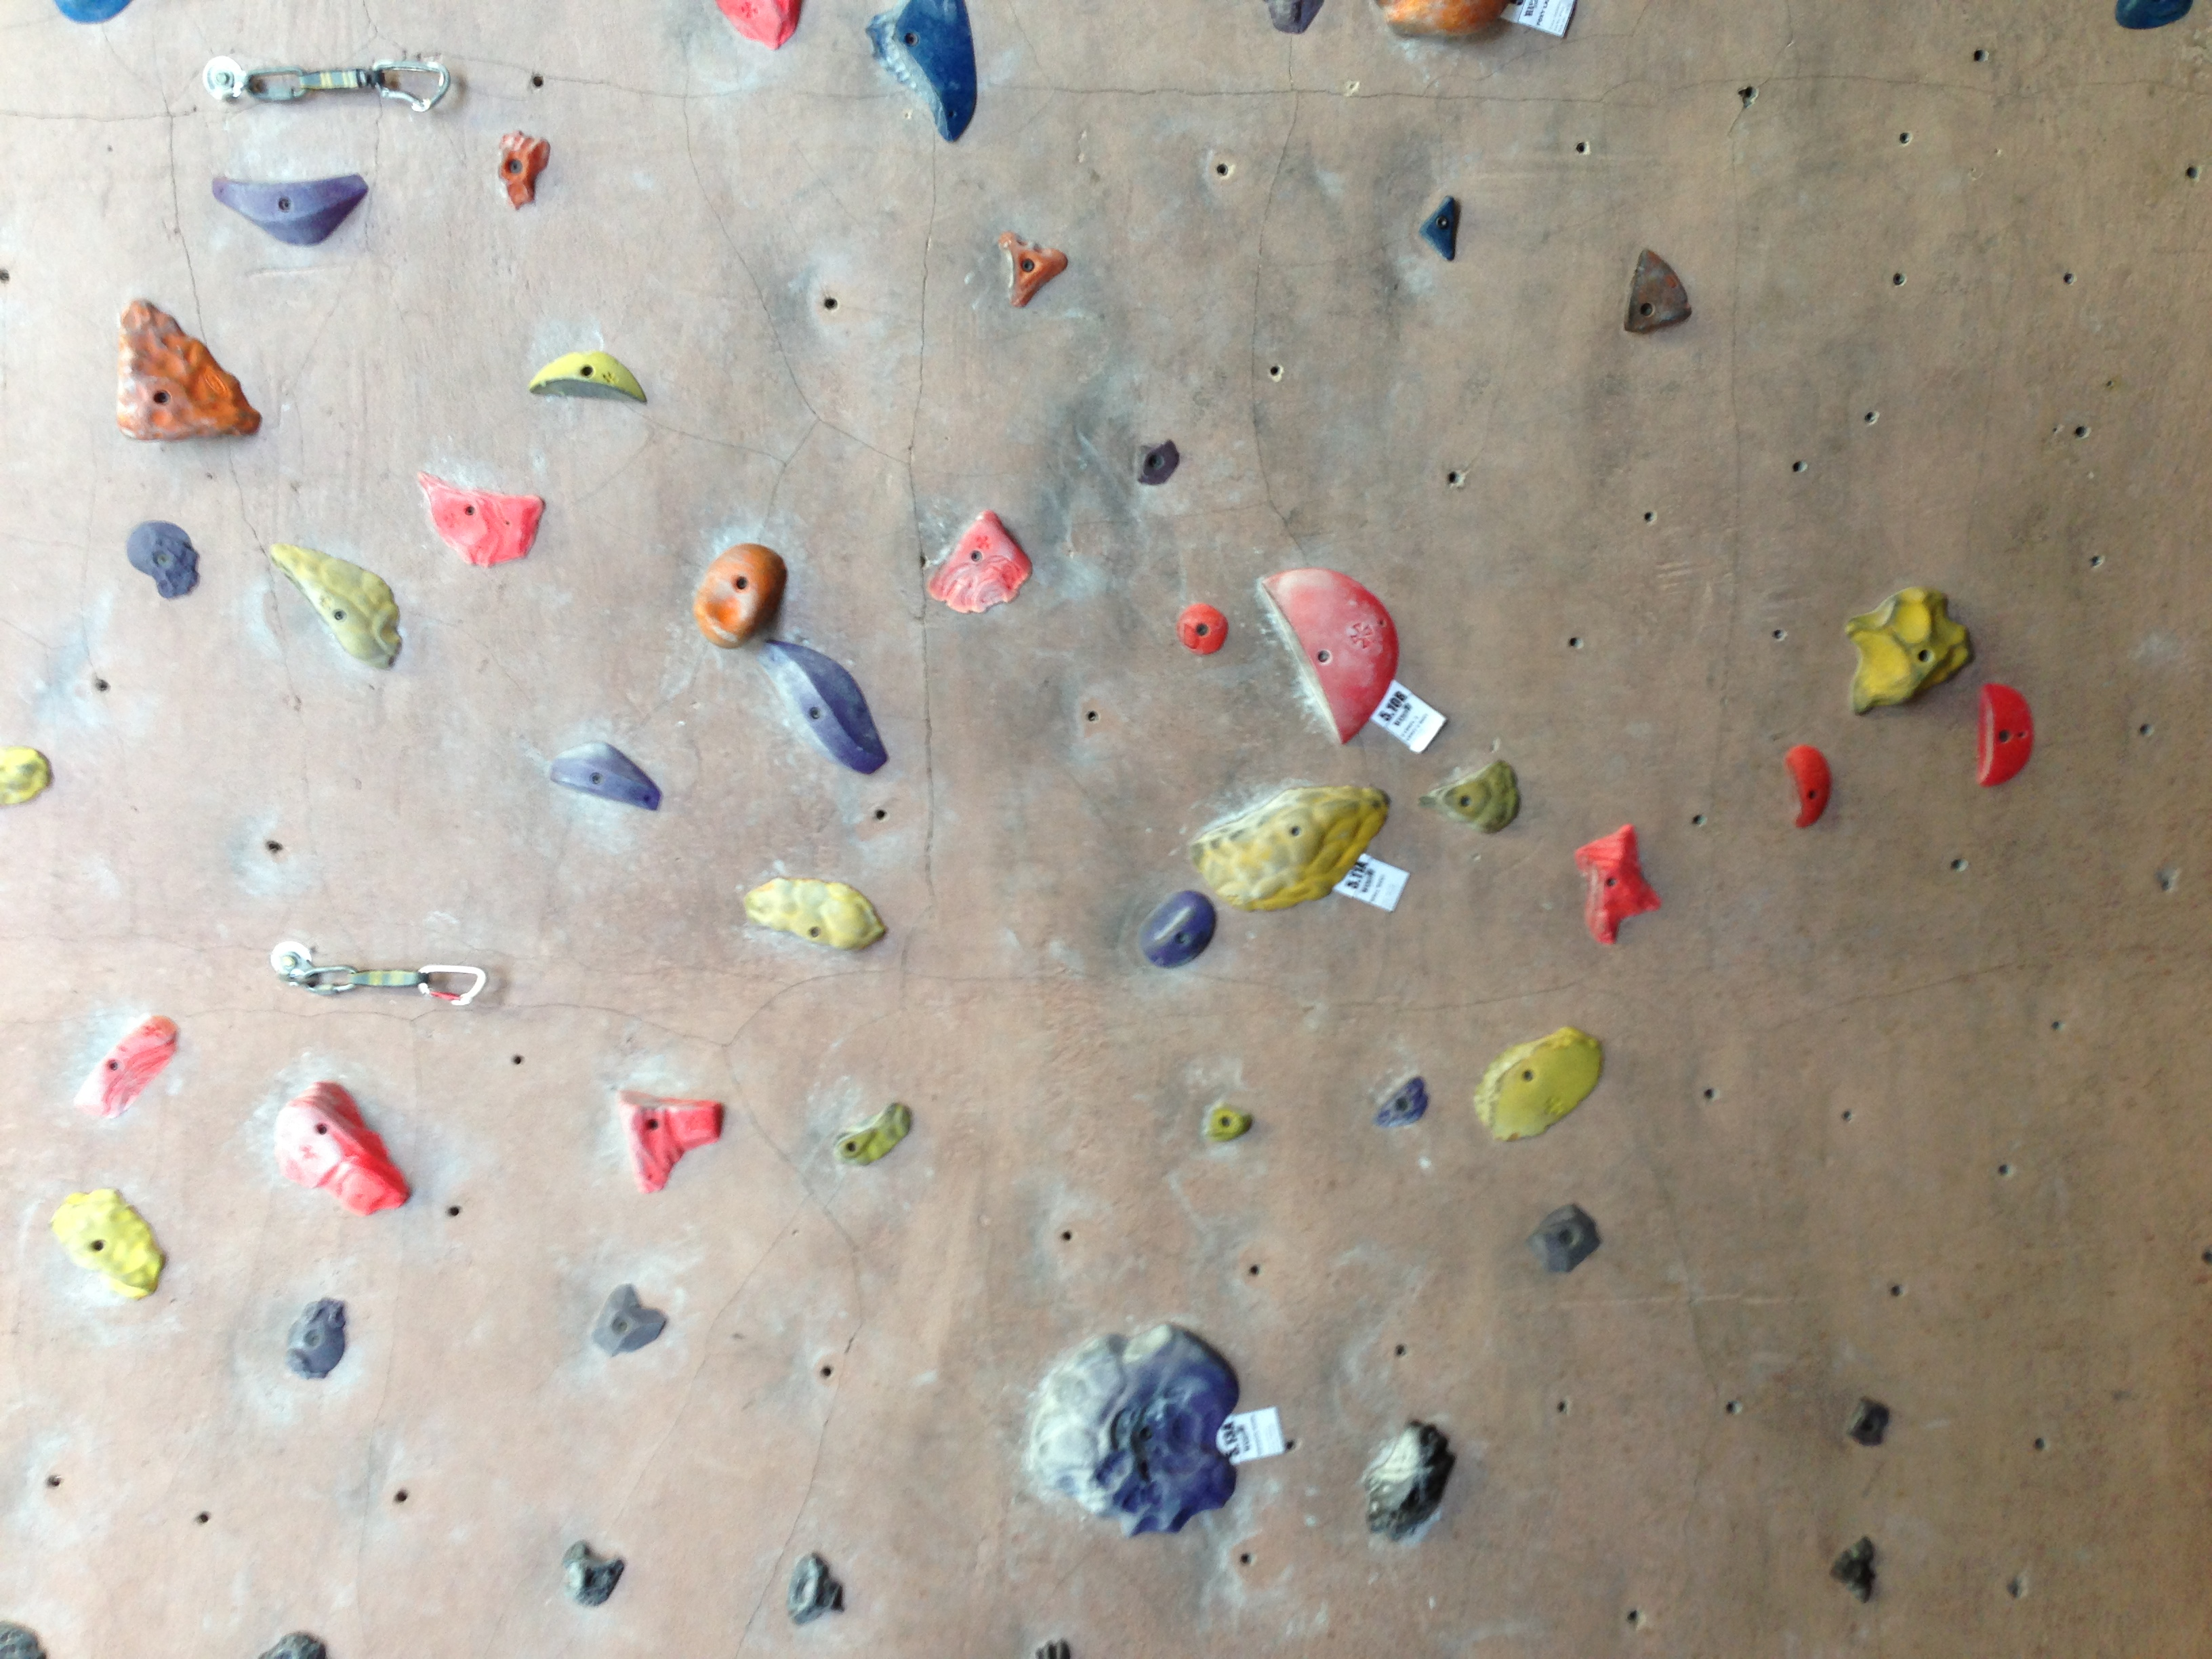
\includegraphics[height=\linewidth,angle=-90]{img/test2.JPG}
\end{column}
\begin{column}[T]{.6\linewidth}
\vspace{.8cm}
Challenges
\pause
\begin{itemize}
 \item Physically-viable arrangements
 \item Balance forces
 \item Minimize muscle strain
 \item Path efficiency
\end{itemize}
\pause
\vspace{.3cm}
Scope Constraints
\begin{itemize}
 \item Motion in 2D plane -- no overhang
 \item Depth correlated to grip size
\end{itemize}
\end{column}

\end{columns}
\end{frame}

\section{Approach Overview}

\begin{frame}[t]{Solution Specifications}
Input:
\begin{itemize}
 \item A low-resolution color photo of a rock wall
 \item Single pixel selection by user that maps to one of the grips in the desired route
\end{itemize}
\vspace{.3cm}
\pause

Output:
\begin{itemize}
 \item A viable path that minimizes a specified cost function
 \item Rendering of climber positions along the solution path
 \item Strain analysis
\end{itemize}

\pause
\vspace{.3cm}
Tools:
\begin{itemize}
 \item OpenCV Library
 \item Qt C++ Framework
\end{itemize}
\end{frame}

\begin{frame}[T]{Pipeline}

\pause

\begin{block}{Image Processing}
\begin{itemize}
 \item Route Detection
 \item Grip Analysis
\end{itemize}
\end{block}

\pause

\begin{block}{Heuristic Analysis}
\begin{itemize}
 \item Modeling Grip Support
\end{itemize}
\end{block}

\pause

\begin{block}{Physics Engine}
\begin{itemize}
 \item Modeling a Human
 \item Simulation Motion
\end{itemize}
\end{block}

\pause

\begin{block}{Path Search}
\begin{itemize}
 \item Starting a Route
 \item BFS \& A$^*$
\end{itemize}
\end{block}

\end{frame}


\section{Image Processing}


\begin{frame}{Image Processing}
\begin{columns}
\begin{column}[T]{.5\linewidth}
\includegraphics<1>[width=\linewidth]{img/test2c.jpg}
\includegraphics<2>[width=\linewidth]{img/hue.jpg}
\includegraphics<3>[width=\linewidth]{img/noisy.jpg}
\includegraphics<4>[width=\linewidth]{img/threshold.jpg}
\includegraphics<5>[width=\linewidth]{img/contour.jpg}
\end{column}


\begin{column}[T]{.5\linewidth}
Steps:
\begin{itemize}
 \pause
 \item Convert to HSV color space
 \pause
 \item Threshold image by hue of user selection
 \pause
 \item Denoise image using dilation \& erosion
 \pause
 \item Represent grips as contour
\end{itemize}
\end{column}

\end{columns}
\end{frame}

\begin{frame}[t]{Grip Analysis}
\begin{center}
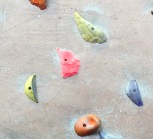
\includegraphics[width=.45\linewidth]{img/close_up.jpg}  \hspace{.05cm}
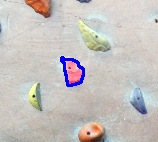
\includegraphics[width=.455\linewidth]{img/close_up_c.jpg}
\end{center}
\pause
Physical Properties:\vspace{-.15cm}
\begin{multicols}{2}
\begin{itemize}
 \item[-] Area
 \item[-] Perimeter
 \item[-] Center of Mass
 \item[-] Convexity Defects
\end{itemize}

\end{multicols}
\end{frame}


\begin{frame}[t]{Grip Analysis}
Orientation Estimation
\begin{center}
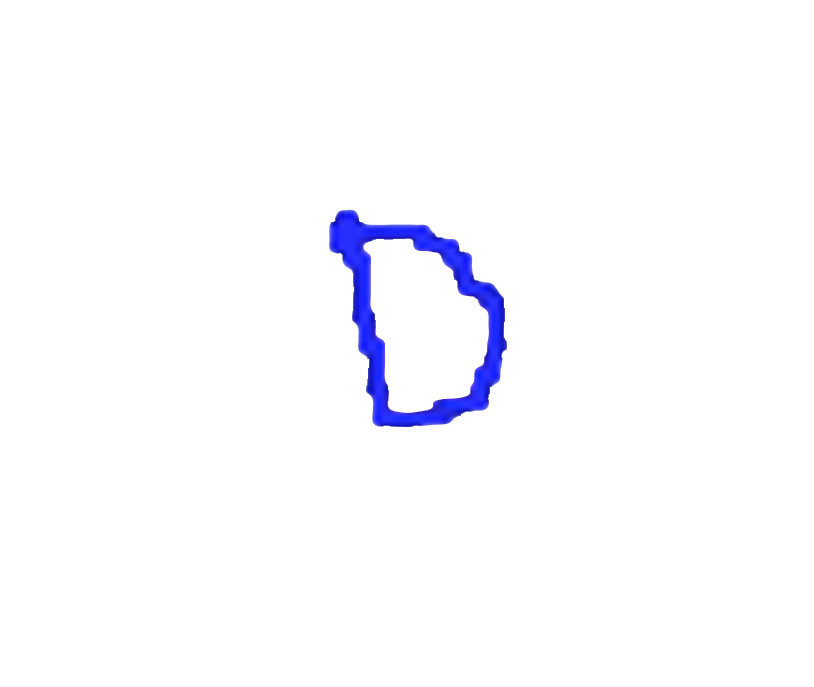
\includegraphics[width=.45\linewidth]{img/pre_normal.jpg}  \hspace{.05cm}
\pause
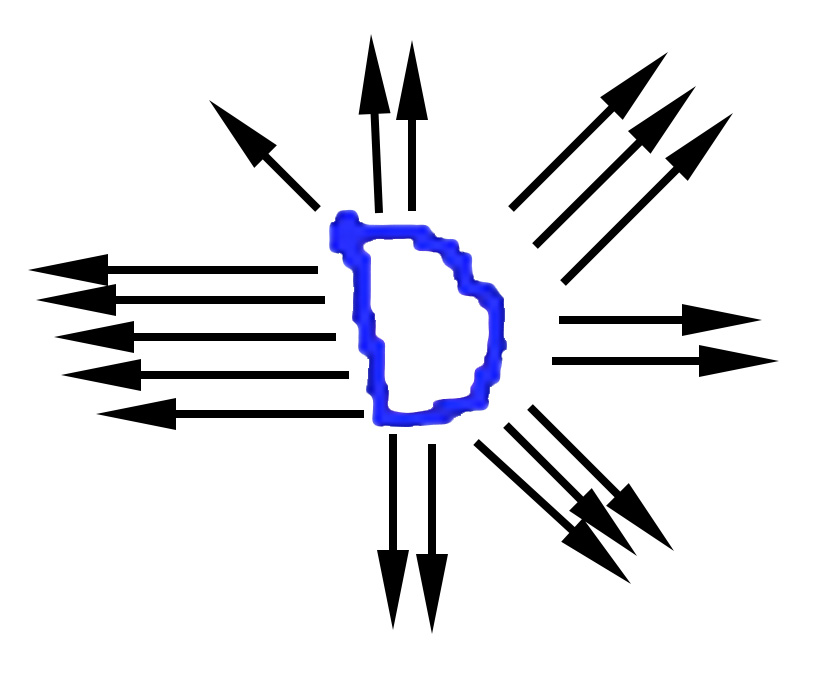
\includegraphics[width=.45\linewidth]{img/normal_field.jpg}
\end{center}

\end{frame}



\section{Heuristic Analysis}
\begin{frame}[t]{Grip Heuristics}
\pause
Binary Criteria:
\begin{itemize}
 \item Can it support a hand or just a foot?
 \item Can it support two limbs?
\end{itemize}
\pause
\vspace{.3cm}
Force as a Continuous Variable:
$$
F = f(a, p, d, N, \theta)
$$
where $a$ is area, $p$ is perimeter, $d$ are the convexity defects, $N$ is the normal field, and $\theta$ is the angle at which the grip is grabbed.\\
\pause
\vspace{.3cm}
As an approximation, 
$$
F = a \cdot N[\theta] + \text{hardlim}(d) \cdot |d|.
$$
\end{frame}

\section{Physics Engine}
\begin{frame}[t]{Physics Engine}
Modeling a Human
\begin{itemize}
 \item 4 point mass limbs
 \item A center of mass, which is not necessarily the geometric center of limbs
 \item Limbs have minimum and maximum distances from center
\end{itemize}

\pause
\vspace{.3cm}
\alert{Challenge is exploring possibilities for the center of mass.}
\end{frame}

\begin{frame}{Center of Mass}
\begin{center}
 \includegraphics<1>[width=.7\linewidth]{img/pos.jpg}
 \includegraphics<2>[width=.7\linewidth]{img/centers.jpg}
 \end{center}
\end{frame}

\section{Path Search}
\begin{frame}[t]{Search}
Constraints
\begin{itemize}
 \item Move one limb at a time
 \item Configuration should be reasonable
 \item Analyze forces and ensure the grips can support the climber
\end{itemize}

\pause
\vspace{.2cm}
Exploration
\begin{itemize}
 \item Allow limbs to be on no grips or to share
 \item Assign strain for each move and for distance of the move
 \item Cost function to minimize strain and maximize height
\end{itemize}

\pause
\vspace{.2cm}
Starting
\begin{itemize}
 \item Search permutations of 4 lowest grips for viable position
 \item Search higher if necessary, provided it can be reached from the ground
\end{itemize}

\end{frame}


\section{Progress}
\begin{frame}[T]{Progress}

\pause
\begin{block}{Image Processing}
\begin{itemize}
 \item Route Detection
 \item Grip Analysis
\end{itemize}
\end{block}


\begin{block}{Heuristic Analysis}
\begin{itemize}
 \item \alert{Modeling Grip Support}
\end{itemize}
\end{block}


\begin{block}{Physics Engine}
\begin{itemize}
 \item Modeling a Human
 \item Simulation Motion
\end{itemize}
\end{block}


\begin{block}{Path Search}
\begin{itemize}
 \item Starting a Route
 \item BFS \& \alert{A$^*$}
\end{itemize}
\end{block}

\end{frame}


\end{document}